\chapter{具体需求}

\section{功能需求}

本产品的主要功能可以分为基本运算、绘制函数图像、初等函数运算、进制转换、组合数学与统计工具、线性代数工具、高等数学工具这七个主要类别。

\textbf{基本运算}

	加、减、乘、除、乘方、开方

\textbf{绘制函数图像}

	可视化函数曲线,支持图像局部放大、缩小功能。

\textbf{初等函数运算}

	幂函数、指数函数、对数函数、三角函数、反三角函数、常数函数等计算求值、代数式相加......

\textbf{进制转换}

	二进制、八进制、十六进制数据格式自由转化

\textbf{组合数学与统计工具}

	组合函数计算,排列与组合的运算;基本统计工具:平均数、求和、统计次数、方差、平方差、中位数、频率统计

\textbf{线性代数工具}

	矩阵运算

\textbf{高等数学工具}

	极限、微分与积分的计算,泰勒展开、常微分方程、FFT的计算......

\subsection{精度}

\subsubsection{输入精度}

本系统对于输入精度无具体要求,只要输入在合法范围内,均可接受。\
如果出现多种精度,计算器将根据数据类型、计算问题等自动化调整。

\subsubsection{传递精度}

对输入数据进行合适的精度和类型的转换,保证中间计算结果的传递过程中不额外引入新的精度损失,将所有合法输入都转换为字符串输出。

\subsubsection{输出精度}

以字符串格式进行输出,保证浮点类型数的精度达到小数点后12位,用户可以指定。

\subsection{时间特性要求}

\subsubsection{程序响应时间}

系统对于一般运算的响应应该在0.1秒之内完成,对于较大数据的响应控制在在1秒之内。

\subsubsection{更新处理时间}

系统的更新处理时间为0.1秒。

\subsubsection{数据的转换和传送时间}

系统运行时,数据转换和传递都应在0.1秒之内完成,数据量较大时,控制在1秒之内完成。

\subsubsection{计算解题时间}

系统的解题时间与计算时间相同,数据量较小时控制在0.1秒内,数据量较大时控制在1秒内。

\subsection{灵活性要求}

\subsubsection{输入方式}

1.本系统接受键盘输入与鼠标点击输入等多种输入方式。

2.支持对输入表达式进行删除、修改、定位。

3.可以回溯之前操作数。

\subsubsection{运行环境的变化}

1.本系统支持windows 7以及之后所有的32位/64位系统。

2.支持MacOS操作系统。

3.支持linux操作系统。

\subsubsection{输出与提示}

本系统能针对不同情况的不合要求的输入产生错误提示信息,并且有帮助信息,方便使用者的正确使用。

\subsubsection{同其他软件的接口}

1.支持从文本为媒介的数据读取,根据命令格式自动进行运算。

2.提供api,可以支持操作系统的调用、穿参。

\subsubsection{精度和有效时限的变化}

1.根据数据精度变化,重新选择合适的策略。

2.自适应调整计算速度。

\subsubsection{计划的变化或改进}

在用户允许下,收集信息,发送至开发者,进行下一步改进。

\subsection{数据管理能力要求}

本系统无数据库,因此对于数据管理的能力无特殊要求。

\subsection{故障处理要求}


\subsubsection{软件故障}

1.容错性,不影响计算结果的错误不会阻止的程序稳定运行。

2.稳定性,当一个进程或其他运行时出错,提供后备措施,尽力保证程序不间断运行。

3.安全性,出现故障,保存计算数据,在错误修复时,提供断点恢复。

\subsubsection{兼容性故障}

若与使用的电脑的操作系统不兼容,则不能使用此系统,该系统运行的系统参考运行环境规定。

\subsubsection{病毒故障}

由于电脑感染病毒而导致该系统不能使用的,解决方法为尝试重新安装。

\subsubsection{硬件故障}

若因硬件问题导致系统无法运行,则应考虑更换相应的硬件设备。

\subsection{用户模式与接口}

本系统提供多种视图给用户,分层次抽象功能,按需提供计算能力。

分为基本模式、绘图模式、科学计算模式、统计模式、数学模式、综合模式


\begin{figure}[ht]
\centering
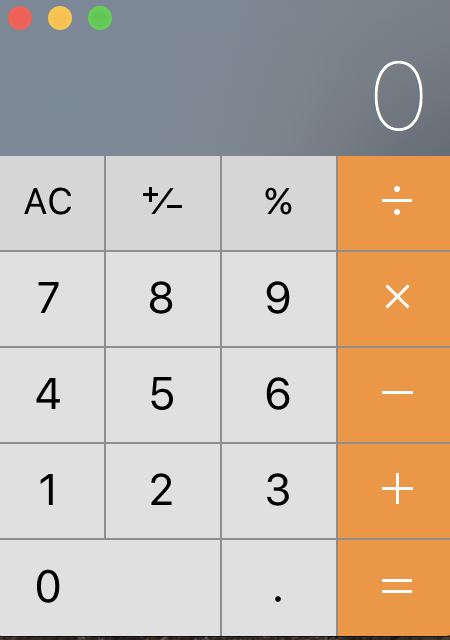
\includegraphics[width=9cm]{basic.png}
\caption{基本视图} \label{fig:basic_conception}
\end{figure}

\begin{figure}[ht]
\centering
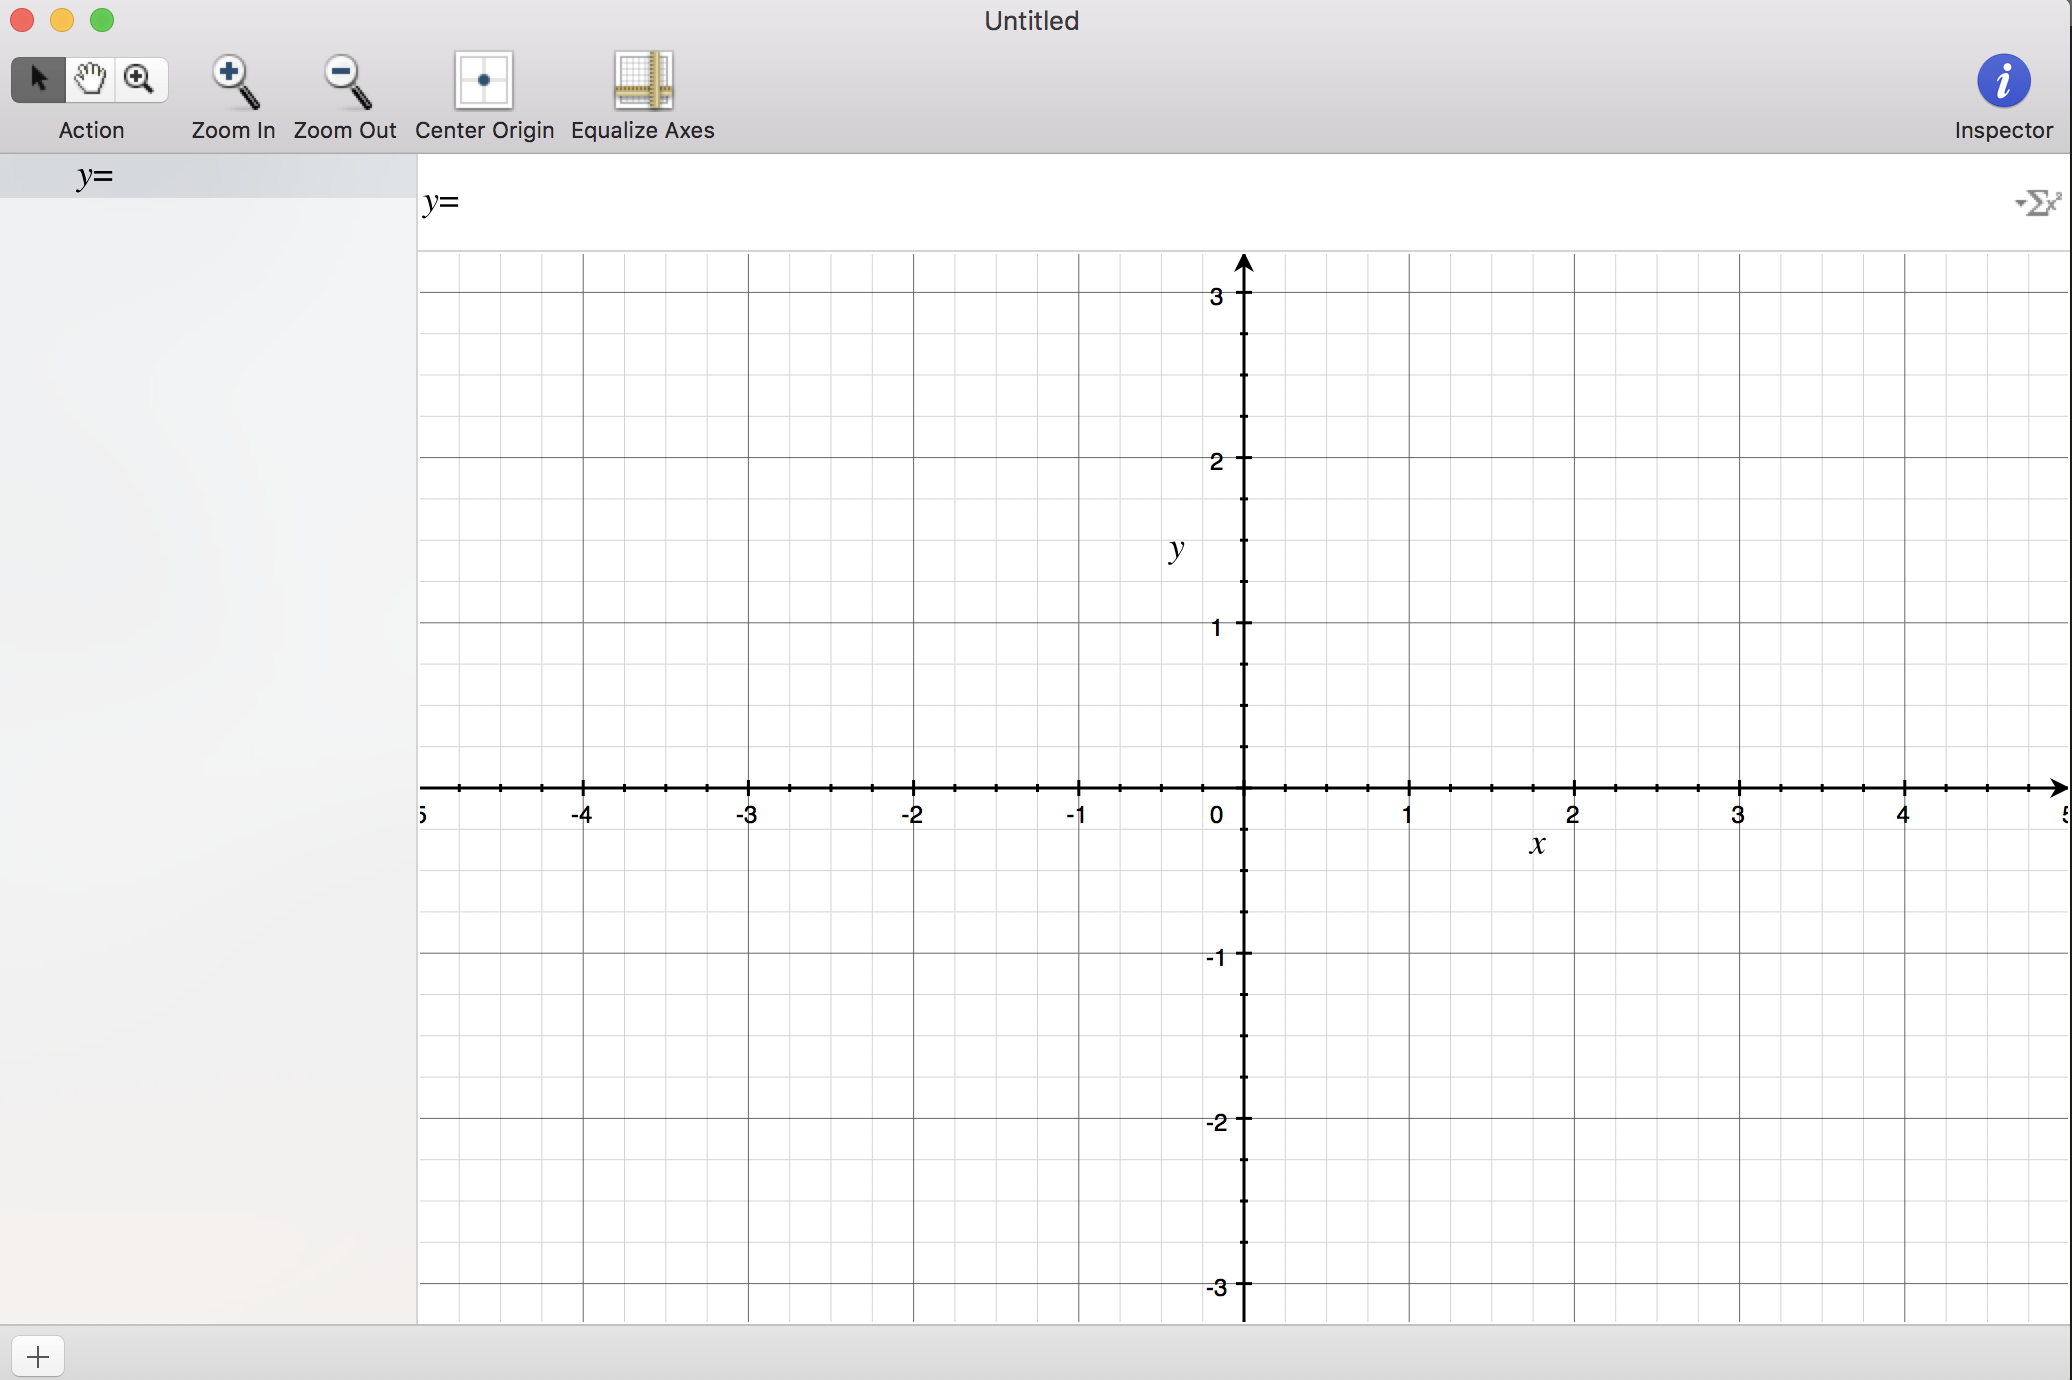
\includegraphics[width=9cm]{draw.png}
\caption{绘图视图} \label{fig:draw_conception}
\end{figure}

\begin{figure}[ht]
\centering
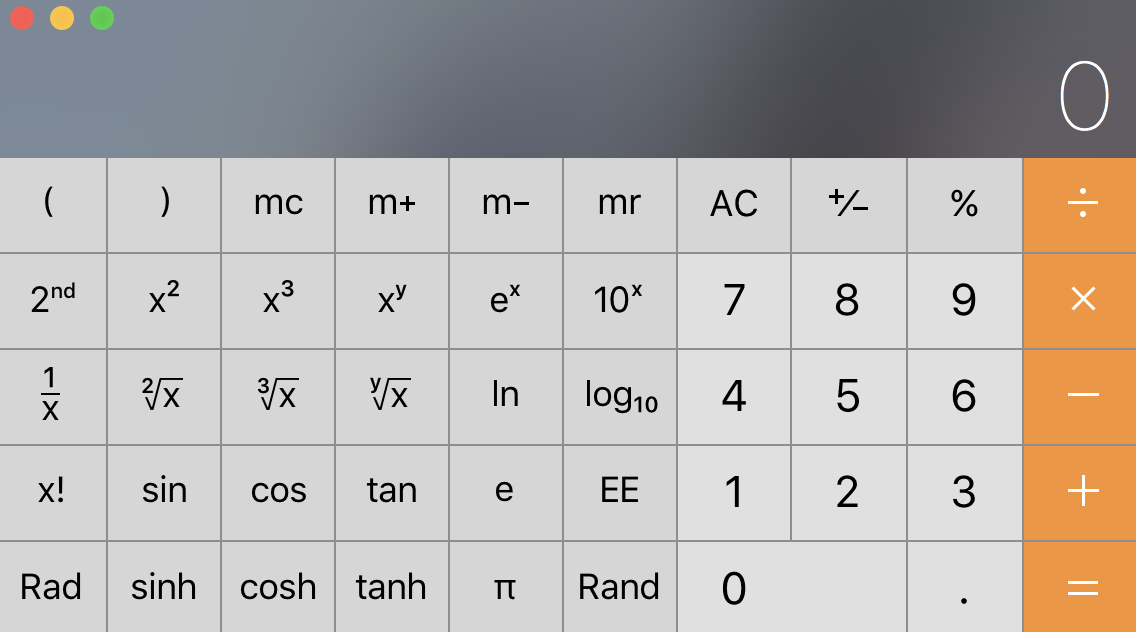
\includegraphics[width=9cm]{scientific.png}
\caption{科学计算} \label{fig:scientific_conception}
\end{figure}


\subsection{其他专门要求}

记录log,方便用户与开发者复查。

